\documentclass[border=6pt,tikz]{standalone}
\usepackage{tikz}
\usepackage{amsmath,amssymb}
\usetikzlibrary{arrows.meta,positioning,fit,backgrounds,calc,shapes.geometric,decorations.pathreplacing,patterns}
\definecolor{ink}{HTML}{1B2430}
\definecolor{muted}{HTML}{6B7785}
\definecolor{accent}{HTML}{2F6FB5}
\definecolor{accent2}{HTML}{C1611F}
\definecolor{good}{HTML}{2E7D5B}
\definecolor{soft}{HTML}{EDF2F7}
\definecolor{soft2}{HTML}{FBEDE2}
\definecolor{soft3}{HTML}{E6F0E9}
\tikzset{
  box/.style={draw=ink,line width=.7pt,rounded corners=2pt,fill=soft,inner sep=4pt,align=center,font=\sffamily\small},
  boxa/.style={box,fill=soft2},
  boxb/.style={box,fill=soft3},
  plain/.style={align=center,font=\sffamily\small,text=ink},
  tiny/.style={align=center,font=\sffamily\scriptsize,text=muted},
  ar/.style={-{Stealth[length=2.4mm]},draw=ink,line width=.7pt},
  arm/.style={-{Stealth[length=2.4mm]},draw=muted,line width=.6pt,dashed},
  nd/.style={circle,draw=ink,line width=.7pt,fill=white,minimum size=7mm,inner sep=0pt,font=\sffamily\scriptsize},
  ndf/.style={nd,fill=soft},
  ndt/.style={nd,fill=soft2},
}

\begin{document}
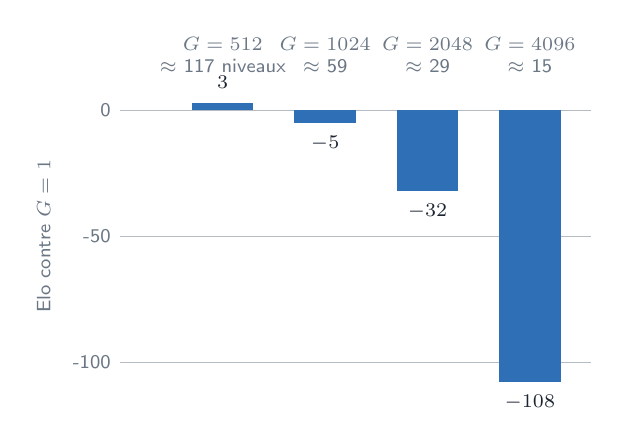
\begin{tikzpicture}[x=13mm,y=0.32mm]
  \draw[muted,line width=.4pt] (0,0) -- (4.6,0);
  \foreach \y in {-100,-50,0} {\draw[muted!50,line width=.3pt] (0,\y) -- (4.6,\y); \node[tiny,left] at (0,\y) {\y};}
  \node[tiny,rotate=90] at (-0.75,-50) {Elo contre $G=1$};
  \foreach \i/\g/\e/\lv in {1/512/3/{$\approx$ 117 niveaux},2/1024/-5/{$\approx$ 59},3/2048/-32/{$\approx$ 29},4/4096/-108/{$\approx$ 15}} {
    \fill[accent] (\i-0.3,0) rectangle (\i+0.3,\e);
    \node[tiny,text=ink] at (\i,{\e<0 ? \e-8 : \e+8}) {$\e$};
    \node[tiny] at (\i,22) {$G=\g$\\\lv};
  }
\end{tikzpicture}
\end{document}
